\section{PreProject}
\subsection{Rich Picture}

\begin{figure}[h!]		%Remember to put the h!, to not fuck the sections.
 \begin{centering}
  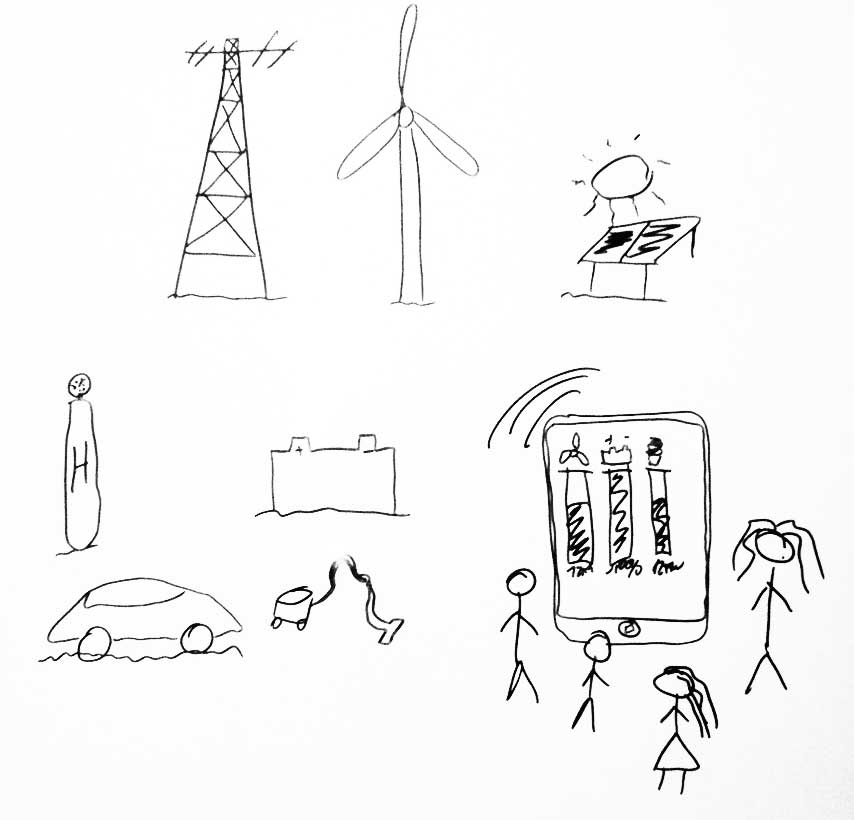
\includegraphics[width=1\textwidth]{images/rich_picture1.png}
   \caption{The surrounding environment is shown in the rich picture. The
 			 elements are: photovoltaic cells, hydrogen storage, battery-charger, wind-turbine
 			 converter, user-interface, the electric grid and different loads such as a
 			 hydrogen engine, vacuum-cleaner etc. }
 \end{centering}
\end{figure}

\subsection{Story Telling}
The main user of the system, Jan Nielsen just got a new energy module to connect to his system. Luckily there is plenty of space
for new modules in the systems energy hub. He connects the device to the hub, where from the administrator web interface he can easily start the module.
The connection of the new modules is straight forward as all the module plugs are similar and the energy hub finds out by itself
if it is an input module, output module or both way module.
\newline
Aarhus University, a place full of innovation and great ideas. Jan welcomes a class of high-school students to the green system simulator. Here it
is possible to see how much energy you can get out of green energy harvesting system
such as wind and solar energy. When the system produces to much energy, the 
energy is stored in form of compressed air. Here people can really come an get an idea about 
how much they can help the environment, but also their own wallet, if they invest in some green energy for their own house.
The guests can navigate around on a screen interface to see how much energy each device 
produces or consumes, this is shown in a down to earth way, where everybody can follow, 
even persons without no special education or courses in the energy field.

\subsection{Story cards}
\textbf{Story Card 1:} Jan is looking at the web interface for the energy hub. From where he can see the status for each modules connected to it
in a graphically way.\\\\
\textbf{Story Card 2:} A new energy module is connected to the hub. Jan opens up the web interface for the energy hub. 
To start, stop or see a more detailed overview of each module, he have to log into the administrator section of the system.
Jan really likes the graphically way that is also kept in the administrator section, this makes it possible for other
non-technically persons to operate the system if Jan is not there one day that the system needs to be operated.\\\\
\textbf{Story Card 3:} It is one of many regularly autumn days in Denmark, rainy and windy. The system is placed outside
but still it operates perfectly under these weather conditions. To operate the system or see the status for one of the modules,
it is not necessary for anyone to go outside to the module, they can simply log onto the system from their workstation pc or laptop.\\\\
\textbf{Story Card 4:} Jan arrives at the university in the morning and an email was send to him reporting a failure in the green energy system, he login to the administrator web interface of the system and he can see what the problem might be, and if it's possible to solve it directly on the interface.
\newpage
\subsection{Preliminary Use Cases}

\begin{figure}[!h]
	\begin{centering}
		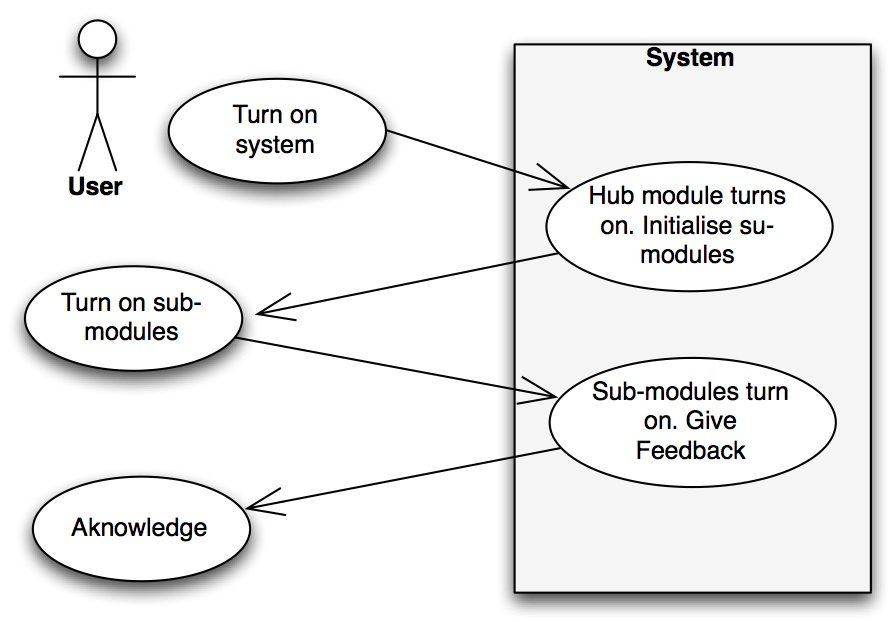
\includegraphics[width=0.7\textwidth]{images/usecases1.jpg}
		\caption{System initialization. }
	\end{centering}
\end{figure}

\begin{figure}[!h]
	\begin{centering}
		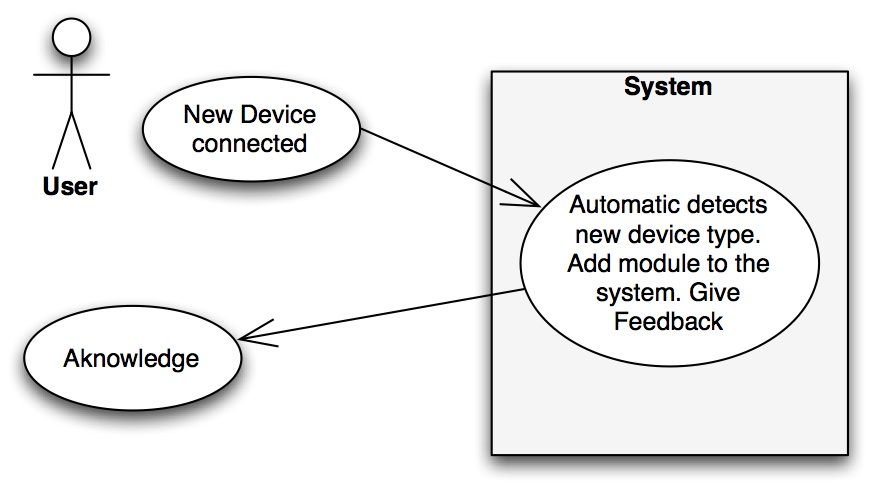
\includegraphics[width=0.7\textwidth]{images/usecases2.jpg}
		\caption{New device connected to the system. }
	\end{centering}
\end{figure}
\newpage

\subsection{Stakeholder Analysis}
This section describes how much influence the different persons
involved in the project have.\\[0.2cm]
\textbf{Project coordinators:}\\ Morten Opprud\\ Klaus Kolle\\
\\
\textbf{Customers/Users:}\\
Jan Nielsen - Customer ( Primary User )\\
High school students ( Secondary Users )\\
Rene A. S. Josefsen ( Web interface customer )\\
\\
\textbf{Developers:}\\
Dennis Madsen\\
Theis Christensen\\
Paulo M. Fontes\\
\\
\textbf{Suppliers:}\\
Jens Mortensen\\
Per Lysgaard\\
\\
\textbf{Theory Advisors:}\\
Henning Slavensky\\
Ulrich Bjerre\\
Kristian Lomholdt\\

\begin{figure}[h!]
 \begin{center}
  \begin{tabular}{| l | l | l |}
   \hline
    & \textbf{Has decision power} & \textbf{Has no decision power} \\ \hline
    \multirow{3}{*}{\textbf{Directly involved stakeholder}} 
    	& Klaus Kolle & Rene A. S. Josefsen\\ 
    	& Morten Opprud &  \\ 
    	& Jan Nielsen &  \\ \hline
    \multirow{2}{*}{\textbf{Not directly involved stakeholders}} 
    	& High School Students & Jens Mortensen\\
    	& Per Lysgaard & \\ \hline
   \end{tabular}
  \end{center}
 \caption{Stakeholder table}
\end{figure}

Klaus Kolle and Morten Opprud, are the project coordinators/managers, they
have decision power over the final product and are directly involved on the
development.\\
\newline
Jan Nielsen is the customer, the primary user of the system so he has the
decision power over the final product and is enroll in all the development
process.\\
\newline
High School Students have decision power over the final interface since they
are the secondary users of the system. They will be our testers.\\
\newline
Rene A. S. Josefsen is our web-interface customer, has no decision power in the
overall system, but is direct involve in the development of the system.\\
\newline
Jens Mortensen is the component supplier, is not directly involved in the
project and has no decision power over the final product.\\
\newline
Per Lysgaard is the money supplier.\\
\newline

\subsection{System Definition}
\textbf{Proposal 1 - Fully automatically}\\
The Energy-Hub system is the central device in the green-energy system. All
inputs and output devices are automatically routed to the right place inside this
device. That means when devices is connected to the Energy Hub, it automatically
detects if it's an input or an output module. On the web interface, the user
have the possibility of using between two modes:
\\ - Green System profile.
\\ - Fast charging profile.
\\The Green profile only makes use of the green power devices such as
photovoltaic-cells, wind power, energy from the charged batteries or from the
compressed oxygen module. 
The fast charging profile on the other hand charges the compressed oxygen module and the
battery on the fastest possible way. In other words, if there is not enough
green energy, energy will be taken from the grid.
\\\\
\textbf{Proposal 2 (Optimizing):}\\
Extra output extension model, so the user can connect devices, and switch
each output on and off. This module will be used to present to high school
students the navigation portal.